\documentclass[aspectratio=169,10pt,t]{beamer}
\usetheme{faeder}

\usepackage{hyperref}
\usepackage{qrcode}
\hypersetup{colorlinks=true,urlcolor=fsTeal,linkcolor=fsNavy}

\graphicspath{{figures/}}
\newcommand{\bngplayground}{https://ruleworld.github.io/bngplayground/}
\newcommand{\notebookurl}{https://github.com/jrfaeder/RBM_Intro_BioNetGen/blob/main/notebooks/stat1_stat3_fitting.ipynb}
\newcommand{\modelfile}[1]{%
  \begin{tikzpicture}[remember picture,overlay]
    \node[anchor=north east,font=\scriptsize,text=fsGray,inner sep=0]
      at ([xshift=-8mm,yshift=-14mm]current page.north east) {File: \texttt{models/#1}};
  \end{tikzpicture}}
\newcommand{\nbsection}[1]{%
  \begin{tikzpicture}[remember picture,overlay]
    \node[anchor=north east,font=\scriptsize,text=fsGray,inner sep=0]
      at ([xshift=-8mm,yshift=-14mm]current page.north east) {Notebook: Section #1};
  \end{tikzpicture}}

\title{Fitting Models to Data}
\subtitle{Module 3: Sensitivity analysis and parameter estimation}
\author{Jim Faeder}
\institute{MSCBIO 2025 \textperiodcentered{} Introduction to Bioinformatics Programming in Python}
\date{Fall 2026}

\begin{document}

% ======================================================================
\begin{frame}[plain]
  \titlepage
\end{frame}

% Resources slide shared by all modules:  % Resources slide shared by all modules:  % Resources slide shared by all modules:  \input{../shared/resources}
\newcommand{\courserepo}{https://github.com/jrfaeder/RBM_Intro_BioNetGen}
\begin{frame}{Resources}
  \begin{columns}[T]
    \begin{column}{0.64\textwidth}
      \begin{itemize}
        \setlength\itemsep{1.5mm}
        \item \textbf{BioNetGen}: software, documentation, and tutorials:
              \href{https://bionetgen.org}{bionetgen.org}
        \item \textbf{VS Code extension}: search the Extensions panel for
              \emph{BioNetGen}
        \item \textbf{bngsim}: fast ODE and stochastic simulation of BioNetGen models
              from Python: \href{https://bngsim.readthedocs.io}{bngsim.readthedocs.io}\\
              Install with \code{pip install bngsim bionetgen}
        \item \textbf{Course repository}:
              \href{\courserepo}{github.com/jrfaeder/RBM\_Intro\_BioNetGen}
          \begin{itemize}
            \item \code{models/} \quad BNGL models used in the slides
            \item \code{notebooks/} \quad Jupyter notebooks for simulation and fitting
            \item \code{Slides/pdf/} \quad slides and handouts
          \end{itemize}
      \end{itemize}
    \end{column}
    \begin{column}{0.32\textwidth}
      \centering
      \vskip2mm
      \qrcode[height=3.4cm]{\courserepo}\\[2mm]
      {\small Course repository}\\
      {\scriptsize\color{fsGray} models, notebooks, slides}
    \end{column}
  \end{columns}
\end{frame}

\newcommand{\courserepo}{https://github.com/jrfaeder/RBM_Intro_BioNetGen}
\begin{frame}{Resources}
  \begin{columns}[T]
    \begin{column}{0.64\textwidth}
      \begin{itemize}
        \setlength\itemsep{1.5mm}
        \item \textbf{BioNetGen}: software, documentation, and tutorials:
              \href{https://bionetgen.org}{bionetgen.org}
        \item \textbf{VS Code extension}: search the Extensions panel for
              \emph{BioNetGen}
        \item \textbf{bngsim}: fast ODE and stochastic simulation of BioNetGen models
              from Python: \href{https://bngsim.readthedocs.io}{bngsim.readthedocs.io}\\
              Install with \code{pip install bngsim bionetgen}
        \item \textbf{Course repository}:
              \href{\courserepo}{github.com/jrfaeder/RBM\_Intro\_BioNetGen}
          \begin{itemize}
            \item \code{models/} \quad BNGL models used in the slides
            \item \code{notebooks/} \quad Jupyter notebooks for simulation and fitting
            \item \code{Slides/pdf/} \quad slides and handouts
          \end{itemize}
      \end{itemize}
    \end{column}
    \begin{column}{0.32\textwidth}
      \centering
      \vskip2mm
      \qrcode[height=3.4cm]{\courserepo}\\[2mm]
      {\small Course repository}\\
      {\scriptsize\color{fsGray} models, notebooks, slides}
    \end{column}
  \end{columns}
\end{frame}

\newcommand{\courserepo}{https://github.com/jrfaeder/RBM_Intro_BioNetGen}
\begin{frame}{Resources}
  \begin{columns}[T]
    \begin{column}{0.64\textwidth}
      \begin{itemize}
        \setlength\itemsep{1.5mm}
        \item \textbf{BioNetGen}: software, documentation, and tutorials:
              \href{https://bionetgen.org}{bionetgen.org}
        \item \textbf{VS Code extension}: search the Extensions panel for
              \emph{BioNetGen}
        \item \textbf{bngsim}: fast ODE and stochastic simulation of BioNetGen models
              from Python: \href{https://bngsim.readthedocs.io}{bngsim.readthedocs.io}\\
              Install with \code{pip install bngsim bionetgen}
        \item \textbf{Course repository}:
              \href{\courserepo}{github.com/jrfaeder/RBM\_Intro\_BioNetGen}
          \begin{itemize}
            \item \code{models/} \quad BNGL models used in the slides
            \item \code{notebooks/} \quad Jupyter notebooks for simulation and fitting
            \item \code{Slides/pdf/} \quad slides and handouts
          \end{itemize}
      \end{itemize}
    \end{column}
    \begin{column}{0.32\textwidth}
      \centering
      \vskip2mm
      \qrcode[height=3.4cm]{\courserepo}\\[2mm]
      {\small Course repository}\\
      {\scriptsize\color{fsGray} models, notebooks, slides}
    \end{column}
  \end{columns}
\end{frame}

\newcommand{\bookchapters}{%
  \bookchapter{07-analysis}{7}{Analyzing models (sensitivity analysis)}
  \item Chapter 9: Parameter estimation {\color{fsGray}(in preparation)}}
% Slide pointing to the companion book, shared by all modules.
% Before % Slide pointing to the companion book, shared by all modules.
% Before % Slide pointing to the companion book, shared by all modules.
% Before \input{../shared/book}, define \bookchapters as itemize entries
% made with \bookchapter{file-stem}{number}{title}.
\newcommand{\bookurl}{https://ruleworld.github.io/bionetgen-book/}
\newcommand{\bookchapter}[3]{%
  \item \href{\bookurl chapters/#1.html}{Chapter #2: #3}}
\begin{frame}{The book}
  \begin{columns}[T]
    \begin{column}{0.64\textwidth}
      \emph{Rule-Based Modeling of Biological Systems: Theory and practice with
      BioNetGen} is an open book that develops the material of this course in
      more depth, with every model, figure, and exercise.\\[1mm]
      \href{\bookurl}{ruleworld.github.io/bionetgen-book}
      \vskip3mm
      For this module, read:
      \begin{itemize}
        \setlength\itemsep{1mm}
        \bookchapters
      \end{itemize}
    \end{column}
    \begin{column}{0.32\textwidth}
      \centering
      \qrcode[height=3cm]{\bookurl}\\[1mm]
      {\small The book}
    \end{column}
  \end{columns}
\end{frame}
, define \bookchapters as itemize entries
% made with \bookchapter{file-stem}{number}{title}.
\newcommand{\bookurl}{https://ruleworld.github.io/bionetgen-book/}
\newcommand{\bookchapter}[3]{%
  \item \href{\bookurl chapters/#1.html}{Chapter #2: #3}}
\begin{frame}{The book}
  \begin{columns}[T]
    \begin{column}{0.64\textwidth}
      \emph{Rule-Based Modeling of Biological Systems: Theory and practice with
      BioNetGen} is an open book that develops the material of this course in
      more depth, with every model, figure, and exercise.\\[1mm]
      \href{\bookurl}{ruleworld.github.io/bionetgen-book}
      \vskip3mm
      For this module, read:
      \begin{itemize}
        \setlength\itemsep{1mm}
        \bookchapters
      \end{itemize}
    \end{column}
    \begin{column}{0.32\textwidth}
      \centering
      \qrcode[height=3cm]{\bookurl}\\[1mm]
      {\small The book}
    \end{column}
  \end{columns}
\end{frame}
, define \bookchapters as itemize entries
% made with \bookchapter{file-stem}{number}{title}.
\newcommand{\bookurl}{https://ruleworld.github.io/bionetgen-book/}
\newcommand{\bookchapter}[3]{%
  \item \href{\bookurl chapters/#1.html}{Chapter #2: #3}}
\begin{frame}{The book}
  \begin{columns}[T]
    \begin{column}{0.64\textwidth}
      \emph{Rule-Based Modeling of Biological Systems: Theory and practice with
      BioNetGen} is an open book that develops the material of this course in
      more depth, with every model, figure, and exercise.\\[1mm]
      \href{\bookurl}{ruleworld.github.io/bionetgen-book}
      \vskip3mm
      For this module, read:
      \begin{itemize}
        \setlength\itemsep{1mm}
        \bookchapters
      \end{itemize}
    \end{column}
    \begin{column}{0.32\textwidth}
      \centering
      \qrcode[height=3cm]{\bookurl}\\[1mm]
      {\small The book}
    \end{column}
  \end{columns}
\end{frame}


\begin{frame}{Goals for this module}
  By the end of this module you should be able to
  \begin{enumerate}[<+->]
    \setlength\itemsep{1.5mm}
    \item say where the parameters of a signaling model come from, and set
          \hl{plausible ranges} when they are unknown
    \item convert between \hl{concentrations and copy numbers}
    \item compute and interpret \hl{local and global sensitivities}
    \item explain the difference between a parameter that affects the outputs and one
          the data can determine (\hl{identifiability})
    \item fit a model by minimizing $\chi^2$ with \hl{multistart optimization}, and judge
          the estimates with \hl{profile likelihoods}
    \item use the model to decide which \hl{new experiment} would help
  \end{enumerate}
\end{frame}

% ======================================================================
\section{Where parameters come from}

\begin{frame}{The modeling cycle}
  \begin{columns}[c]
    \begin{column}{0.5\textwidth}
      \centering
      \begin{tikzpicture}[
          box/.style={draw=fsNavy,fill=fsLight,rounded corners=3pt,text width=3.1cm,
                      align=center,font=\small,minimum height=11mm},
          arr/.style={-{Stealth[length=2mm]},fsNavy,line width=0.8pt}]
        \node[box] (b) at (0,2) {1. Build a model from known and hypothesized interactions};
        \node[box,fill=fsGold!25,draw=fsGold] (c) at (4,2) {2. \textbf{Calibrate} parameters to data};
        \node[box] (a) at (4,0) {3. Analyze the model to find new behaviors};
        \node[box] (t) at (0,0) {4. Do experiments to test predictions};
        \draw[arr] (b) -- (c); \draw[arr] (c) -- (a); \draw[arr] (a) -- (t); \draw[arr] (t) -- (b);
      \end{tikzpicture}
    \end{column}
    \begin{column}{0.46\textwidth}
      \small
      \begin{itemize}[<+->]
        \setlength\itemsep{1.5mm}
        \item Model behavior depends on its \textbf{structure} (the rules) and its
              \textbf{parameters}.
        \item Two kinds of parameters: \textbf{amounts} (copy numbers, concentrations)
              and \textbf{rate constants}.
        \item Some can be measured directly. The rest must be \hl{inferred from data}:
              find the parameters that make the model reproduce the measurements.
        \item This module: how to tell which parameters matter, which ones data can
              determine, and how to estimate them.
      \end{itemize}
    \end{column}
  \end{columns}
\end{frame}

\begin{frame}{Parameters are gleaned from many sources}
  \begin{columns}[T]
    \begin{column}{0.5\textwidth}
      \small
      \begin{tabular}{@{}ll@{}}
        \toprule
        kind & typical source \\
        \midrule
        physical constants, volumes & textbooks, imaging \\
        protein copy numbers & quantitative proteomics, \\
                             & flow cytometry, westerns \\
        binding constants & SPR, ITC, other biophysics \\
        catalytic rates & enzyme assays \\
        everything else & \hl{fitting to dynamic data} \\
        \bottomrule
      \end{tabular}
    \end{column}
    \begin{column}{0.46\textwidth}
      \onslide<2->
      \small
      In the 2003 model of Fc$\varepsilon$RI signaling, protein amounts came from
      antibody-based measurements, receptor binding kinetics from biophysical
      experiments, and the remaining rate constants from western blots of
      phosphorylation kinetics.
      \vskip2mm
      \onslide<3->
      Here we assume the \textbf{copy numbers are known} and estimate only the
      \textbf{rate constants}, a common situation now that proteomics gives copy
      numbers for most signaling proteins.
    \end{column}
  \end{columns}
  \source{Faeder et al., \emph{J.\ Immunol.}\ \textbf{170}, 3769 (2003)}
\end{frame}

\begin{frame}[fragile]{Copy numbers: counting molecules per cell}
  \modelfile{stat1\_stat3.bngl}
  \begin{columns}[T]
    \begin{column}{0.52\textwidth}
      \small
      \begin{itemize}[<+->]
        \setlength\itemsep{1.2mm}
        \item Concentration $c$ (M) in volume $V$ (L) $\;\to\;$ copy number $c\,N_A V$.
        \item First-order rate constants (s$^{-1}$) need no conversion.
        \item Second-order $k$ (M$^{-1}$s$^{-1}$) $\;\to\;$ $k/(N_A V)$ per pair of
              molecules, where $V$ is the volume in which they meet.
        \item Ligand meets receptors from the medium: $V_\text{ext} = 1/\rho_\text{cell}$,
              the medium volume per cell. Docking happens in the cytoplasm
              ($V_\text{cyt}\approx 1$ pL), promoter binding in the nucleus.
      \end{itemize}
      \vskip1mm
      \onslide<5->
      {\footnotesize Check: $k_\text{on}[L] = 10^7 \times 10^{-9} = 10^{-2}$ s$^{-1}$ in
      either set of units.}
    \end{column}
    \begin{column}{0.45\textwidth}
      \onslide<1->
\begin{lstlisting}[language=bngl,basicstyle=\ttfamily\scriptsize]
NA         6.022e23
Vcyt       1e-12         # L
cell_dens  1e9           # cells/L
Vext       1/cell_dens   # L per cell
L_conc     1e-9          # M
L0         L_conc*NA*Vext   # 6.0e5
S3_0       2e5           # 0.33 uM
kon        1e7           # 1/M/s
kon_m      kon/(NA*Vext) # 1.7e-8 /s
kS3on      1e6           # 1/M/s
kS3on_m    kS3on/(NA*Vcyt)  # 1.7e-6 /s
\end{lstlisting}
      {\scriptsize Rate constants stay in standard units, which is what we fit; the model
      converts them.}
    \end{column}
  \end{columns}
\end{frame}

\begin{frame}[fragile]{The model: STAT1 and STAT3 compete for the receptor}
  \modelfile{stat1\_stat3.bngl}
\begin{lstlisting}[language=bngl,basicstyle=\ttfamily\scriptsize]
S1bind:   R(l!+,s) + STAT1(r,Y~0) -> R(l!+,s!1).STAT1(r!1,Y~0)            kS1on_m
S3bind:   R(l!+,s) + STAT3(r,Y~0) -> R(l!+,s!1).STAT3(r!1,Y~0)            kS3on_m
S3act:    R(l!+,socs,s!1).STAT3(r!1,Y~0) -> R(l!+,socs,s!1).STAT3(r!1,Y~P)  kact
Gbind:    STAT3(r,Y~P,g) + G(s) <-> STAT3(r,Y~P,g!1).G(s!1)               kGon_m, kGoff
SOCSbind: R(l!+,socs) + SOCS(r) -> R(l!+,socs!1).SOCS(r!1)                kSOCSon_m
\end{lstlisting}
  \begin{itemize}[<+->]
    \setlength\itemsep{1.2mm}
    \item Built from Module 2, version 3, with a second STAT.
    \item STAT1 and STAT3 dock at the same receptor site, and the receptor kinase
          phosphorylates either one.
    \item Only pSTAT3 binds the \emph{SOCS3} promoter, and SOCS3 blocks the kinase for
          both STATs: STAT3 drives the feedback that shuts off STAT1 too.
    \item Roughly the situation for IL-6, which signals mostly through STAT3.
    \item 18 rate constants, 29 species, 65 reactions.
  \end{itemize}
\end{frame}

\begin{frame}{Dynamics with the ``true'' parameters}
  \modelfile{stat1\_stat3.bngl}
  \centering
  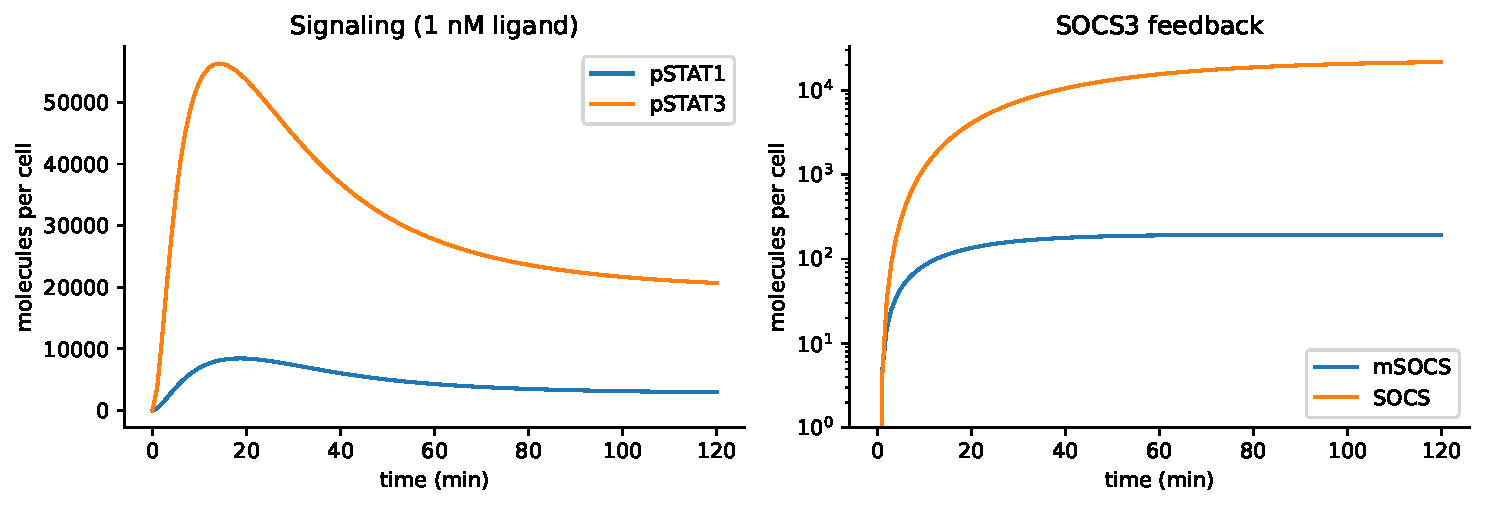
\includegraphics[width=0.84\linewidth]{model_dynamics.pdf}
  \raggedright
  \begin{itemize}[<2->]
    \item pSTAT3 peaks at about 14 min, at 28\% of total STAT3. pSTAT1 peaks at 8\% of
          STAT1, because STAT3 wins most of the docking sites.
    \item SOCS3 reaches about $2\times10^4$ copies, more than the 5000 receptors, and holds
          both responses down.
  \end{itemize}
\end{frame}

\begin{frame}{Plausible ranges come from the class of process}
  \nbsection{1}
  Before fitting, say where each rate constant could lie, \emph{without} looking at
  particular values:
  \vskip2mm
  \centering
  \small
  \begin{tabular}{@{}lll@{}}
    \toprule
    class & parameters & range \\
    \midrule
    association & \code{kon}, \code{kS1on}, \code{kS3on}, \code{kGon}, \code{kSOCSon}
      & $10^{4}$--$10^{8}$ M$^{-1}$s$^{-1}$ \\
    dissociation & \code{koff}, \code{kS1off}, \code{kS3off}, \code{kGoff}, \code{kSOCSoff}
      & $10^{-4}$--$10^{1}$ s$^{-1}$ \\
    catalysis, synthesis & \code{kact}, \code{kdiss}, \code{ktx}, \code{ktl}
      & $10^{-3}$--$10^{1}$ s$^{-1}$ \\
    decay & \code{kS1dephos}, \code{kS3dephos}, \code{kmdeg}, \code{kSOCSdeg}
      & $10^{-5}$--$10^{-2}$ s$^{-1}$ \\
    \bottomrule
  \end{tabular}
  \vskip3mm
  \raggedright
  \begin{itemize}[<2->]
    \item Association: slow protein binding up to near the diffusion limit. Decay:
          half-lives from a minute to a day.
    \item Work in $\log_{10} k$: a step of 0.1 is the same relative change at any scale.
  \end{itemize}
\end{frame}

\begin{frame}{Test the method on synthetic data}
  \nbsection{2}
  \begin{columns}[T]
    \begin{column}{0.46\textwidth}
      \small
      \begin{itemize}[<+->]
        \setlength\itemsep{1.5mm}
        \item Choose ``true'' rate constants and simulate pSTAT1 and pSTAT3 after
              1 nM ligand.
        \item Sample 15 time points over 2 hours and add noise: SD = 10\% of the value
              + 200 molecules.
        \item Then forget the true values, and see how many we can recover.
        \item With real data there is no answer key. Synthetic data tell us what the
              method can and cannot do.
      \end{itemize}
    \end{column}
    \begin{column}{0.5\textwidth}
      \onslide<1->
      \centering
      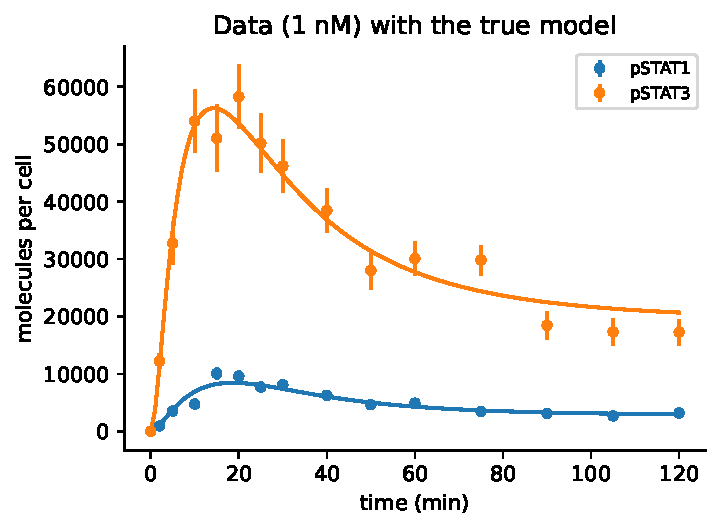
\includegraphics[width=\linewidth]{data_high.pdf}
    \end{column}
  \end{columns}
\end{frame}

% ======================================================================
\section{Sensitivity analysis}

\begin{frame}{Which parameters matter?}
  \begin{itemize}[<+->]
    \setlength\itemsep{2mm}
    \item A \textbf{parameter scan} varies one or two parameters over a range and
          follows the outputs. It maps out behaviors, but does not scale to 18 parameters.
    \item \textbf{Sensitivity analysis} measures the effect of every parameter on the
          outputs of interest.
    \item Goals: find the parameters with the \hl{most} effect, and those with the
          \hl{least}. Use this to guide estimation and experiments.
    \item \textbf{Local}: small changes around one parameter set (derivatives).
    \item \textbf{Global}: all parameters varied together over their plausible ranges.
  \end{itemize}
\end{frame}

\begin{frame}{Local sensitivity}
  \nbsection{3a}
  \begin{columns}[T]
    \begin{column}{0.52\textwidth}
      Sensitivity of output $O_i$ to parameter $p_j$:
      \[
        S_{ij}(t) = \frac{\partial \ln O_i(t)}{\partial \ln p_j}
                  = \frac{p_j}{O_i}\frac{\partial O_i}{\partial p_j}
      \]
      \small
      $S = 0.5$: a 1\% increase in $p_j$ raises $O_i$ by 0.5\%. Independent of units.
    \end{column}
    \begin{column}{0.44\textwidth}
      \small
      \onslide<2->
      \textbf{Finite differences}: rerun with $p_j \to (1+\epsilon)p_j$; one extra
      simulation per parameter, and $\epsilon$ must be chosen with care.
      \vskip2mm
      \onslide<3->
      \textbf{Forward sensitivity equations}: integrate
      \[
        \frac{d}{dt}\frac{\partial \mathbf{x}}{\partial p_j}
        = \frac{\partial \mathbf{f}}{\partial \mathbf{x}}\frac{\partial \mathbf{x}}{\partial p_j}
          + \frac{\partial \mathbf{f}}{\partial p_j}
      \]
      alongside $\dot{\mathbf{x}} = \mathbf{f}(\mathbf{x};\mathbf{p})$. Exact, in one run:
      \code{Simulator(..., sensitivity\_params=[...])} in bngsim.
    \end{column}
  \end{columns}
\end{frame}

\begin{frame}{Local sensitivities of pSTAT1 and pSTAT3}
  \nbsection{3a}
  \centering
  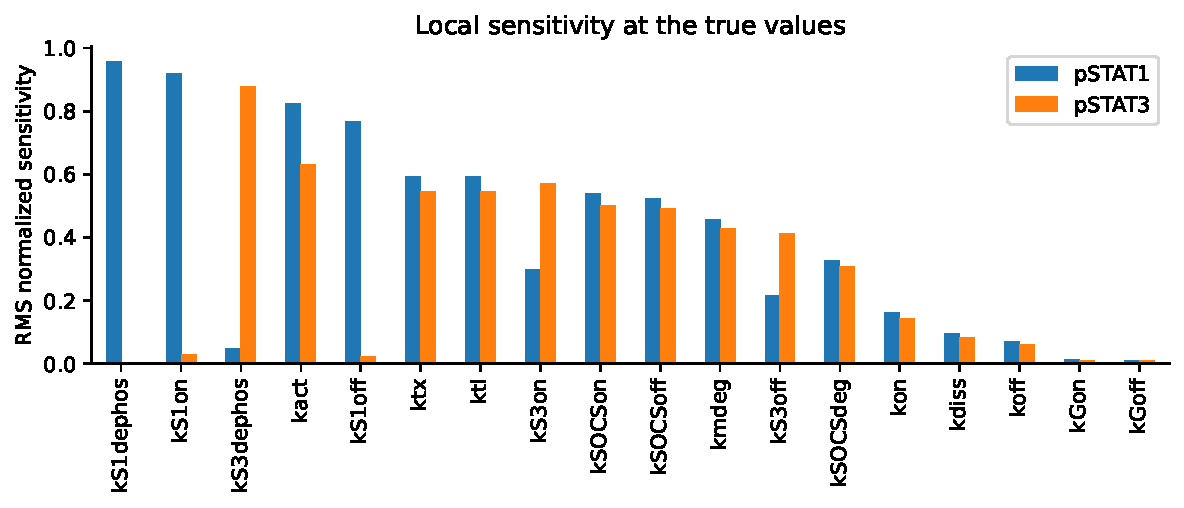
\includegraphics[width=0.62\linewidth]{local_bar.pdf}
  \vskip1mm
  \raggedright
  \small
  \begin{itemize}[<2->]
    \item Each STAT's own dephosphorylation rate dominates its response.
    \item Docking and \code{kact} set the level. Competition: \code{kS3on} \emph{lowers}
          pSTAT1 ($S\approx-0.3$).
    \item \code{ktx} and \code{ktl} are identical. Promoter binding and ligand binding barely
          matter: both are saturated.
  \end{itemize}
\end{frame}

\begin{frame}{Sensitivities change over time}
  \nbsection{3a}
  \centering
  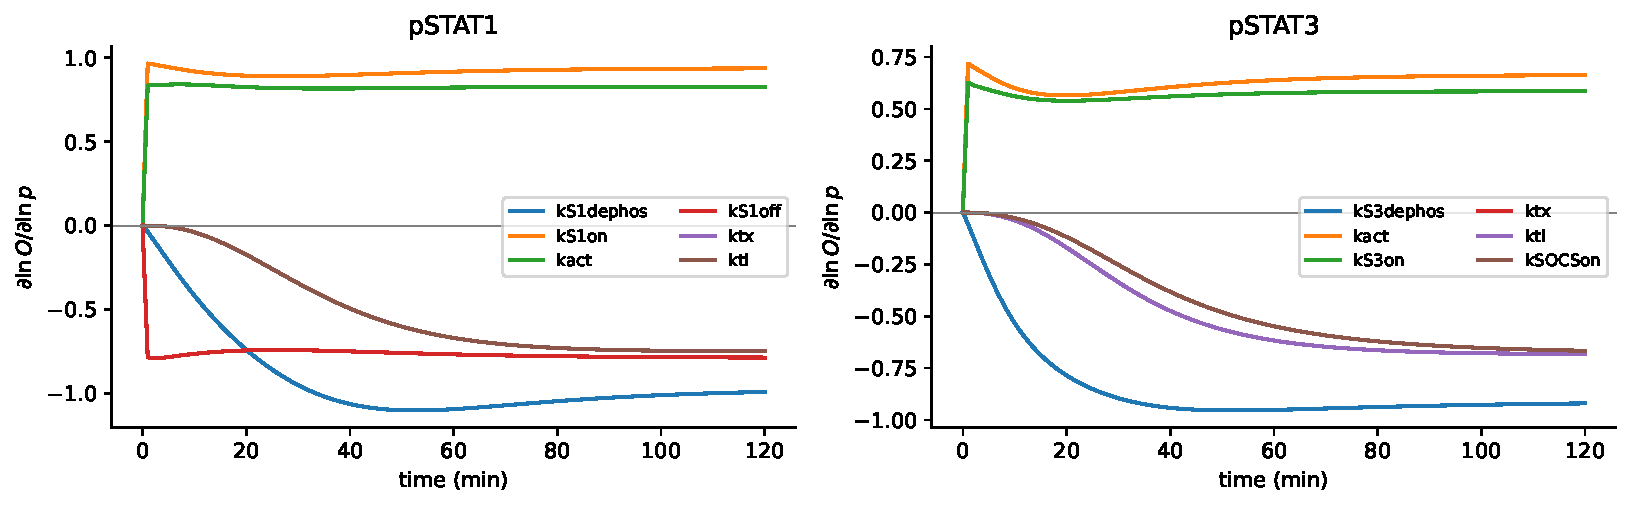
\includegraphics[width=0.9\linewidth]{local_time.pdf}
  \raggedright
  \small
  \begin{itemize}[<2->]
    \item Docking and kinase rates matter from the start; the SOCS3 loop
          (\code{ktx}, \code{ktl}, \code{kSOCSon}) only after about 20 min, once SOCS3 has
          accumulated.
  \end{itemize}
\end{frame}

\begin{frame}{Global sensitivity: sample the whole range}
  \nbsection{3b}
  \begin{columns}[T]
    \begin{column}{0.5\textwidth}
      \small
      \begin{enumerate}[<+->]
        \setlength\itemsep{1.5mm}
        \item Draw $N$ parameter sets in $\log_{10}$ space by \textbf{Latin hypercube
              sampling}: each range is cut into $N$ strata, each used once.
        \item Simulate each set and compute output features: peak, time of peak,
              value at 60 min.
        \item Regress each (log) feature on the (log) parameters, both standardized:
              $\tilde{O} \approx \sum_j \beta_j\,\tilde{p}_j$.
              The \textbf{standardized regression coefficients} $\beta_j$ rank the
              parameters; $R^2$ says how much a linear model explains.
      \end{enumerate}
    \end{column}
    \begin{column}{0.46\textwidth}
      \onslide<4->
      \small
      \begin{block}{Why log space?}
        Rate constants spread over orders of magnitude. Sampling uniformly in linear
        space puts 90\% of the samples in the top decade and washes out the rest.
      \end{block}
      \vskip2mm
      \onslide<5->
      2000 simulations of this model take a few seconds.
    \end{column}
  \end{columns}
\end{frame}

\begin{frame}{Global sensitivities}
  \nbsection{3b}
  \begin{columns}[T]
    \begin{column}{0.48\textwidth}
      \centering
      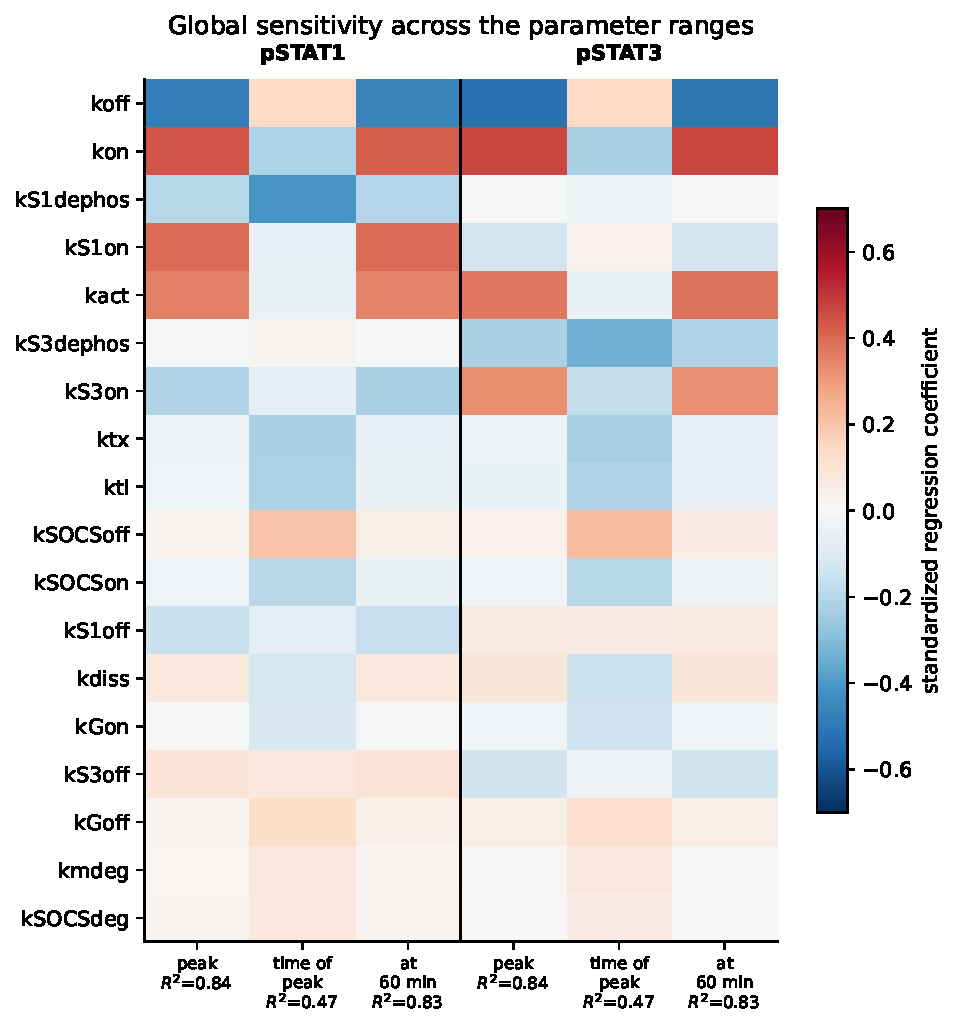
\includegraphics[height=0.68\textheight]{global_src.pdf}
    \end{column}
    \begin{column}{0.48\textwidth}
      \small
      \begin{itemize}[<2->]
        \setlength\itemsep{1.5mm}
        \item \textbf{Ligand binding ranks first}, although it barely mattered
          locally. Across the ranges binding is often slow or weak, and then receptor
          occupancy limits everything.
        \item Dephosphorylation, docking, and \code{kact} matter in both analyses.
        \item Some locally important parameters (\code{kS1off}, the SOCS3 loop) average
          out globally.
        \item Peak and 60 min value: $R^2\approx 0.84$. Time of peak: $R^2\approx 0.47$,
          shaped by interactions a linear model misses.
      \end{itemize}
    \end{column}
  \end{columns}
\end{frame}

% ======================================================================
\section{Identifiability}

\begin{frame}{Sensitive is not the same as identifiable}
  \begin{itemize}[<+->]
    \setlength\itemsep{2mm}
    \item A parameter can strongly affect the outputs and still not be determined by
          the data, because other parameters can \hl{compensate} for it.
    \item \textbf{Structural} non-identifiability: no data of this kind, however good,
          can determine the parameter. In our model, the outputs depend on \code{ktx}
          and \code{ktl} only through their product: doubling one and halving the other
          changes nothing.
    \item \textbf{Practical} non-identifiability: the parameter could be determined in
          principle, but these data, with this noise, do not constrain it.
    \item Both kinds can be diagnosed from the model, before any fitting.
  \end{itemize}
\end{frame}

\begin{frame}{The Fisher information matrix}
  \nbsection{4}
  \begin{columns}[T]
    \begin{column}{0.5\textwidth}
      For data $y_k$ with standard deviations $\sigma_k$:
      \[
        \mathrm{FIM} = J^\mathsf{T}J, \qquad
        J_{kj} = \frac{1}{\sigma_k}\frac{\partial y_k}{\partial \log_{10} p_j}
      \]
      \small
      \onslide<2->
      \begin{itemize}
        \item Built from sensitivities at the data time points.
        \item Eigenvectors: \textbf{combinations} of parameters.
        \item Eigenvalue $\lambda$: how well the data constrain that combination.
              Standard error $\approx 1/\sqrt{\lambda}$ in $\log_{10}$ units.
      \end{itemize}
    \end{column}
    \begin{column}{0.46\textwidth}
      \onslide<3->
      \small
      \begin{tabular}{@{}rl@{}}
        \toprule
        $\lambda$ & combination known to within \\
        \midrule
        100 & factor of 1.26 \\
        1 & factor of 10 \\
        $10^{-4}$ & not at all \\
        \bottomrule
      \end{tabular}
      \vskip3mm
      \onslide<4->
      Needs no data, only the planned measurements and their noise, so it can
      evaluate an experiment \hl{before} you do it.
    \end{column}
  \end{columns}
\end{frame}

\begin{frame}{Signaling models are sloppy}
  \nbsection{4}
  \centering
  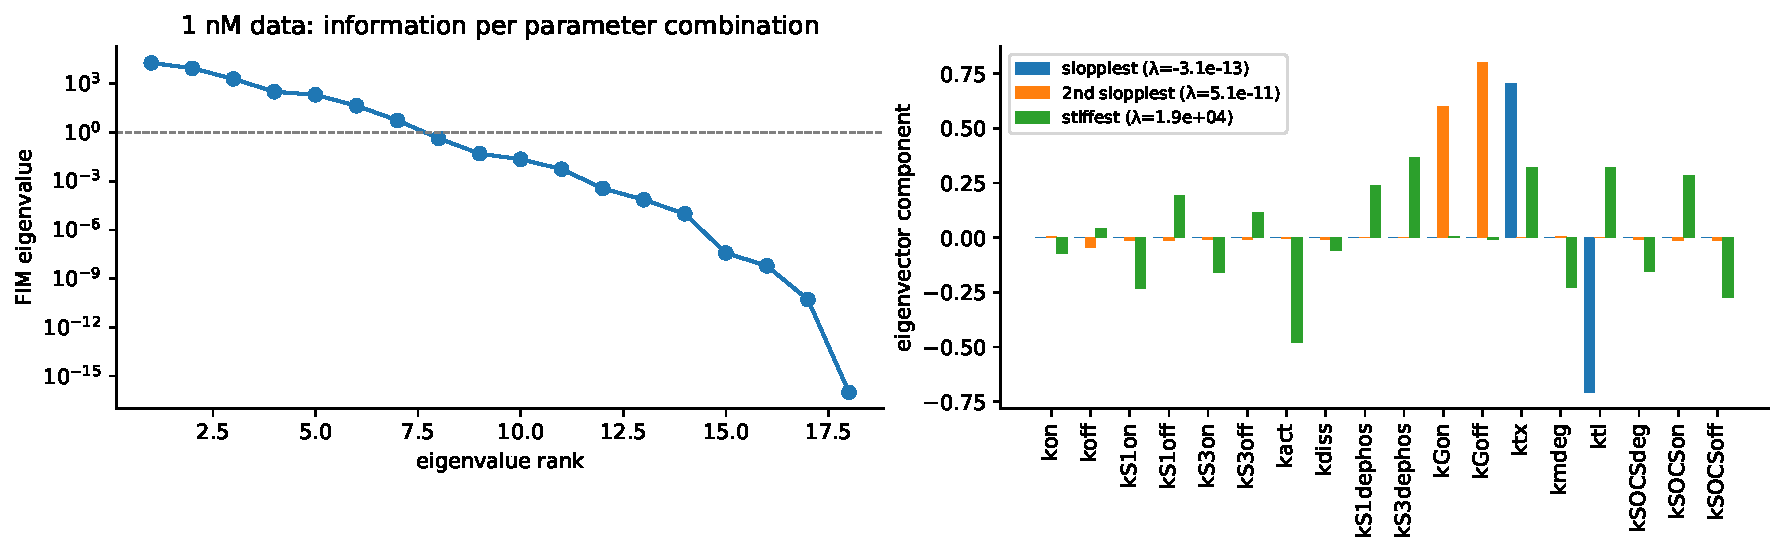
\includegraphics[width=0.95\linewidth]{fim_high.pdf}
  \raggedright
  \small
  \begin{itemize}[<2->]
    \item Eigenvalues span 17 decades; only 7 of 18 combinations exceed 1.
    \item Sloppiest: \code{ktx}$-$\code{ktl}, a \textbf{structural} non-identifiability
          (only the product matters). Next: promoter binding, which is saturated.
  \end{itemize}
  \source{Gutenkunst et al., \emph{PLoS Comput.\ Biol.}\ \textbf{3}, e189 (2007)}
\end{frame}

% ======================================================================
\section{Parameter estimation}

\begin{frame}{Estimation as optimization}
  \begin{columns}[T]
    \begin{column}{0.52\textwidth}
      Find the parameters $\mathbf{p}$ that minimize a \textbf{cost function}.
      \vskip2mm
      \onslide<2->
      Sum of squares: $\displaystyle C(\mathbf{p}) = \sum_k \big(y_k(\mathbf{p}) - y_k^\text{obs}\big)^2$
      \vskip2mm
      \onslide<3->
      With measurement errors $\sigma_k$:
      \[
        \chi^2(\mathbf{p}) = \sum_k \left(\frac{y_k(\mathbf{p}) - y_k^\text{obs}}{\sigma_k}\right)^2
        = -2\ln P(\text{data}\mid\mathbf{p}) + \text{const}
      \]
      for independent Gaussian errors. Minimizing $\chi^2$ is maximizing the likelihood.
    \end{column}
    \begin{column}{0.44\textwidth}
      \onslide<4->
      \small
      \begin{block}{Is the fit good?}
        For a correct model, $\chi^2 \approx N - M$ ($N$ data points, $M$ fitted
        parameters). The probability of a larger $\chi^2$ by chance is
        $Q = 1 - \Gamma\!\left(\frac{N-M}{2}, \frac{\chi^2}{2}\right)$.
      \end{block}
      \onslide<5->
      Meaningful only if the $\sigma_k$ are reliable, which in systems biology they
      often are not.
    \end{column}
  \end{columns}
\end{frame}

\begin{frame}{Optimizers}
  \begin{columns}[T]
    \begin{column}{0.48\textwidth}
      \small
      \textbf{Gradient-free}
      \begin{itemize}
        \item Nelder--Mead simplex
        \item genetic algorithms, differential evolution
        \item particle swarm
      \end{itemize}
      Robust, but need many evaluations.
      \vskip2mm
      \onslide<2->
      \textbf{Gradient-based}
      \begin{itemize}
        \item steepest descent, conjugate gradient, L-BFGS
        \item Newton: fit a quadratic, step to its minimum
        \item for sums of squares: Gauss--Newton, Levenberg--Marquardt, trust region
      \end{itemize}
    \end{column}
    \begin{column}{0.48\textwidth}
      \onslide<3->
      \small
      \begin{block}{Gradients from sensitivities}
        For $\chi^2$ the residuals are $r_k = (y_k - y^\text{obs}_k)/\sigma_k$, and their
        Jacobian $\partial r_k/\partial p_j$ is the same scaled sensitivity matrix $J$
        as in the FIM. Least-squares methods use $J$ to approximate the curvature:
        $\nabla^2\chi^2 \approx 2J^\mathsf{T}J$.
      \end{block}
      \onslide<4->
      With forward sensitivities, each optimizer step costs about one simulation.
    \end{column}
  \end{columns}
\end{frame}

\begin{frame}{Multistart: the landscape has many minima}
  \nbsection{5}
  \centering
  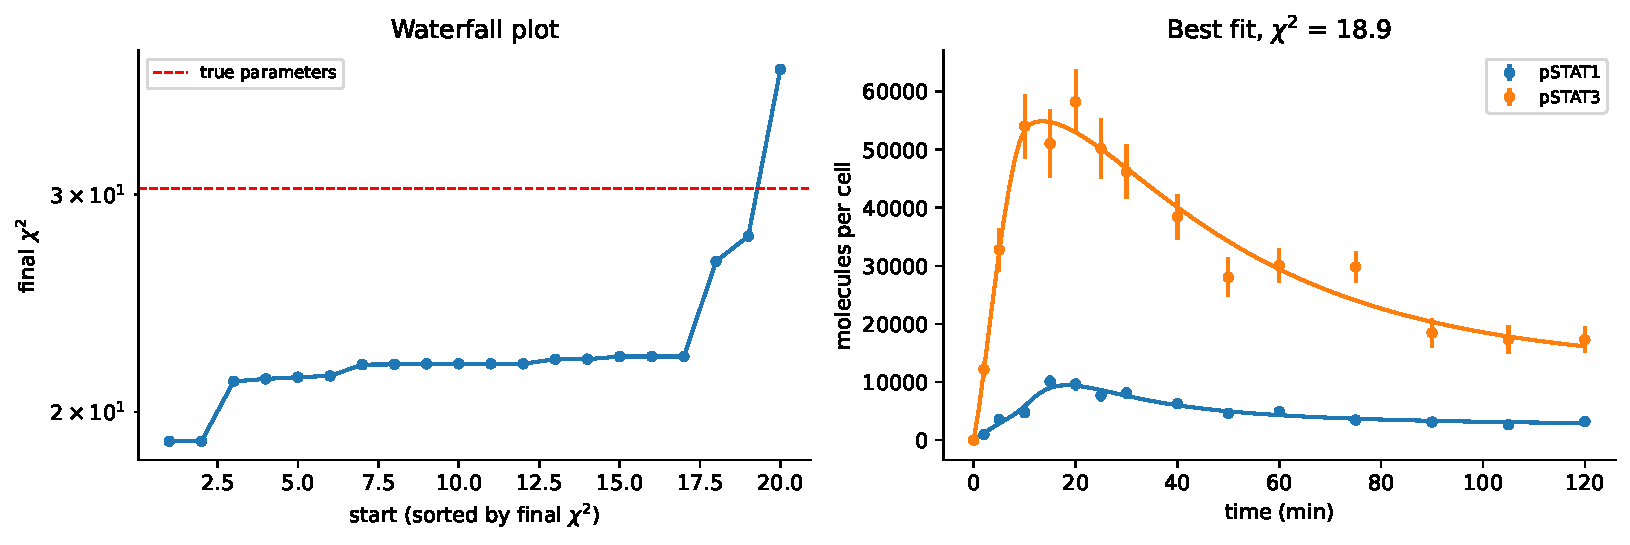
\includegraphics[width=0.85\linewidth]{fit_high.pdf}
  \raggedright
  \small
  \begin{itemize}[<2->]
    \item 17 of 20 starts reach nearly the same $\chi^2$. Best fit: $\chi^2 = 18.9$,
          \emph{below} the 30.3 of the true parameters: the fit follows the noise.
  \end{itemize}
\end{frame}

\begin{frame}{A good fit does not mean good estimates}
  \nbsection{5}
  \centering
  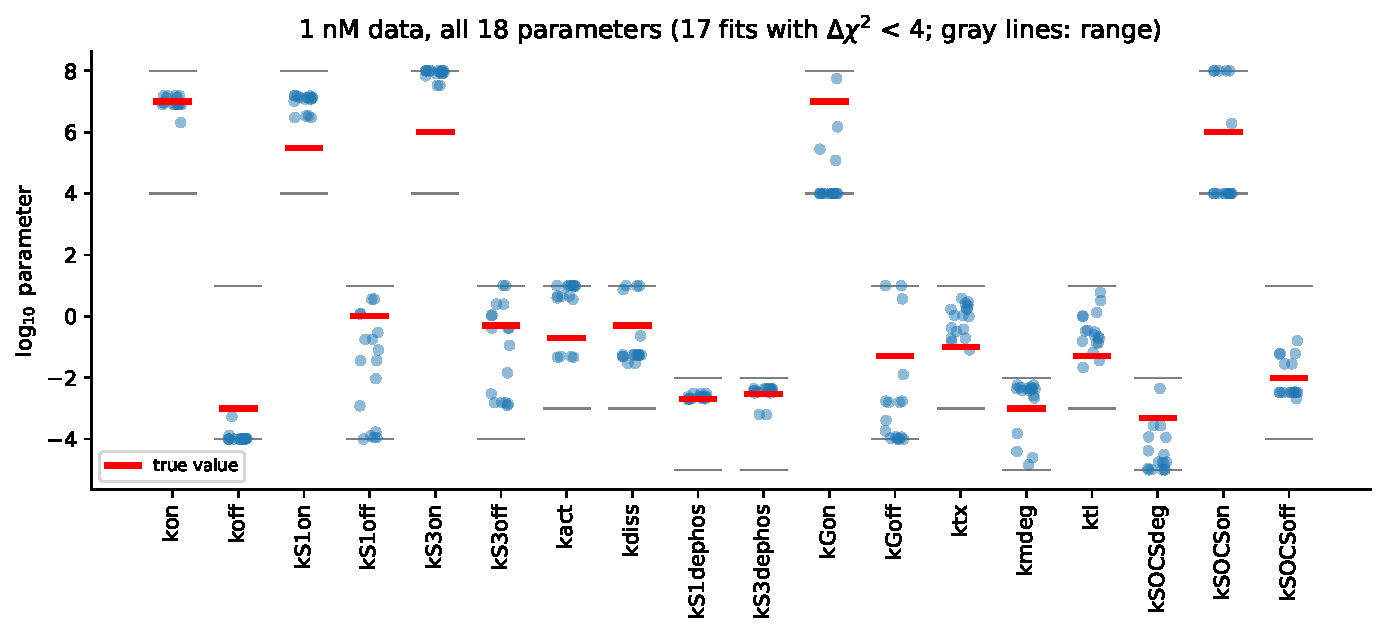
\includegraphics[width=0.7\linewidth]{recovery_high.pdf}
  \raggedright
  \small
  \begin{itemize}[<2->]
    \item Only \code{kS1dephos} is pinned down. \code{kS3on} and \code{koff} sit at
          bounds in every good fit; docking off-rates and the SOCS3 loop scatter.
    \item As the FIM predicted: about 7 combinations are constrained, not 18.
  \end{itemize}
\end{frame}

\begin{frame}{Profile likelihood}
  \nbsection{6}
  \begin{columns}[T]
    \begin{column}{0.5\textwidth}
      Fix $p_i$ at a series of values; at each one, re-optimize everything else:
      \[
        \mathrm{PL}(p_i) = \min_{p_{j\neq i}} \chi^2(\mathbf{p})
      \]
      \small
      \onslide<2->
      The 95\% confidence interval is where $\mathrm{PL}$ stays within 3.84 of its
      minimum ($\chi^2$ with one degree of freedom).
    \end{column}
    \begin{column}{0.46\textwidth}
      \small
      \onslide<3->
      \begin{tikzpicture}[x=1cm,y=1cm]
        \draw[->] (0,0) -- (4.2,0) node[below left,font=\scriptsize] {$\log p_i$};
        \draw[->] (0,0) -- (0,2.4) node[left,font=\scriptsize] {$\Delta\chi^2$};
        \draw[dashed,fsGray] (0,0.9) -- (4,0.9) node[right,font=\tiny] {3.84};
        \draw[fsNavy,line width=1.2pt] (0.4,2.2) parabola bend (1.4,0.05) (2.4,2.2);
        \node[font=\scriptsize,fsNavy] at (1.4,2.5) {identifiable};
        \draw[fsAccent,line width=1.2pt] (2.6,2.2) .. controls (2.9,0.2) .. (3.2,0.06) -- (4,0.04);
        \node[font=\scriptsize,fsAccent] at (3.4,2.5) {one-sided};
      \end{tikzpicture}
      \vskip2mm
      A profile that stays flat to a bound means the data put no limit on the
      parameter in that direction: the others compensate.
    \end{column}
  \end{columns}
  \source{Raue et al., \emph{Bioinformatics} \textbf{25}, 1923 (2009)}
\end{frame}

\begin{frame}{Profiles for four parameters}
  \nbsection{6}
  \centering
  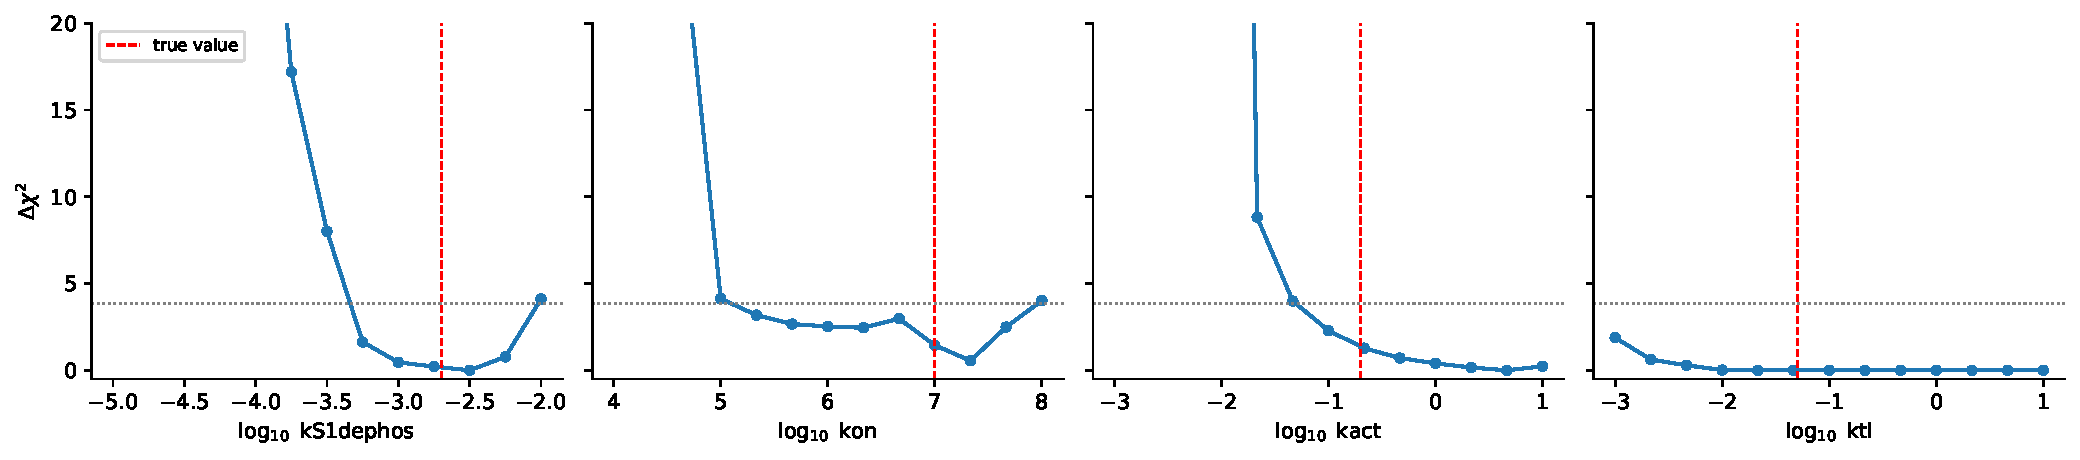
\includegraphics[width=0.9\linewidth]{profiles_high.pdf}
  \raggedright
  \small
  \begin{itemize}[<2->]
    \item \code{kS1dephos}: bounded on both sides, true value inside the 95\% interval.
    \item \code{kon}, \code{kact}: bounded below only. Slow binding and a slow kinase are
          ruled out; faster values fit about as well.
    \item \code{ktl}: flat. \code{ktx} always compensates.
  \end{itemize}
\end{frame}

\begin{frame}{A tempting shortcut: fix the insensitive parameters}
  \nbsection{7}
  \centering
  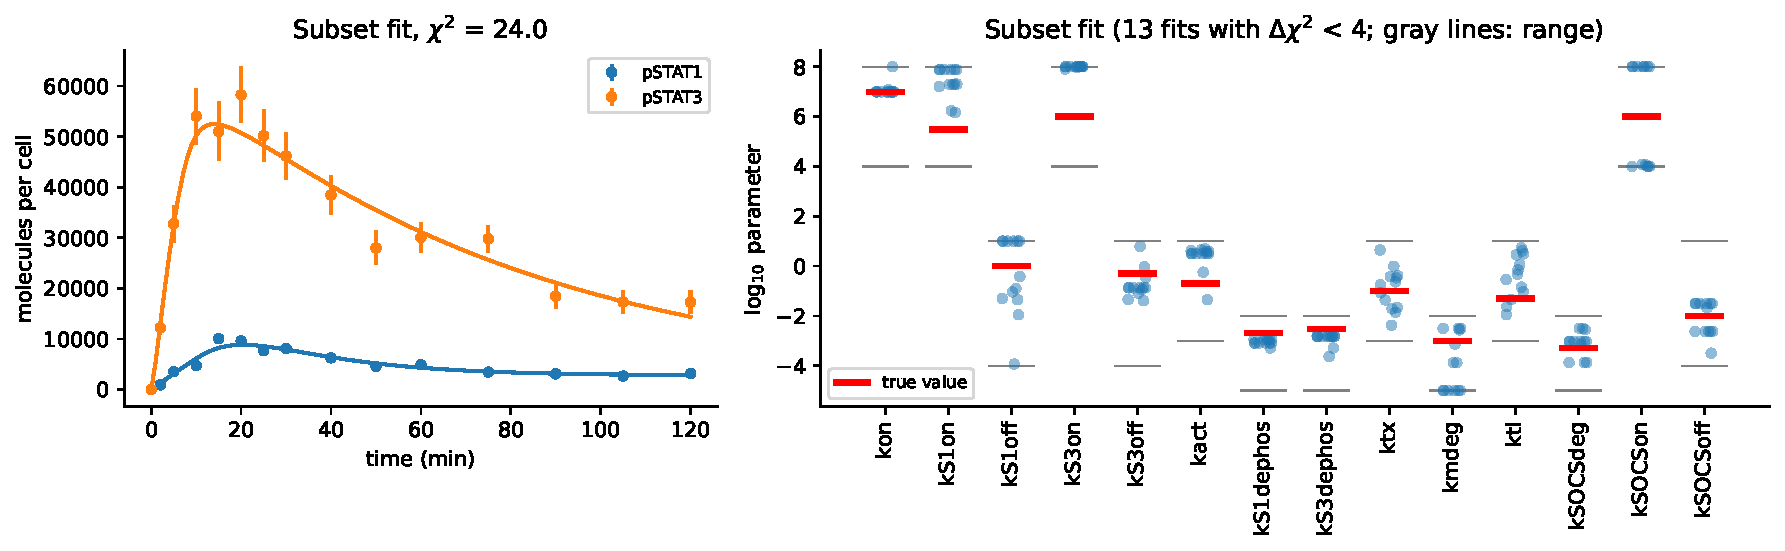
\includegraphics[width=0.95\linewidth]{subset_fit.pdf}
  \raggedright
  \small
  \begin{itemize}[<2->]
    \item Fixed \code{koff}, \code{kdiss}, \code{kGon}, \code{kGoff} (locally
          insensitive) at range centers. Fit almost as good: $\chi^2 = 24.0$ vs.\ 18.9.
    \item But \code{koff} is now 30$\times$ too high, receptors are only $\sim$25\%
          occupied, and other parameters (\code{kact}) compensate. Biased, with no warning.
  \end{itemize}
\end{frame}

\begin{frame}{Design the next experiment with the model}
  \nbsection{8}
  \centering
  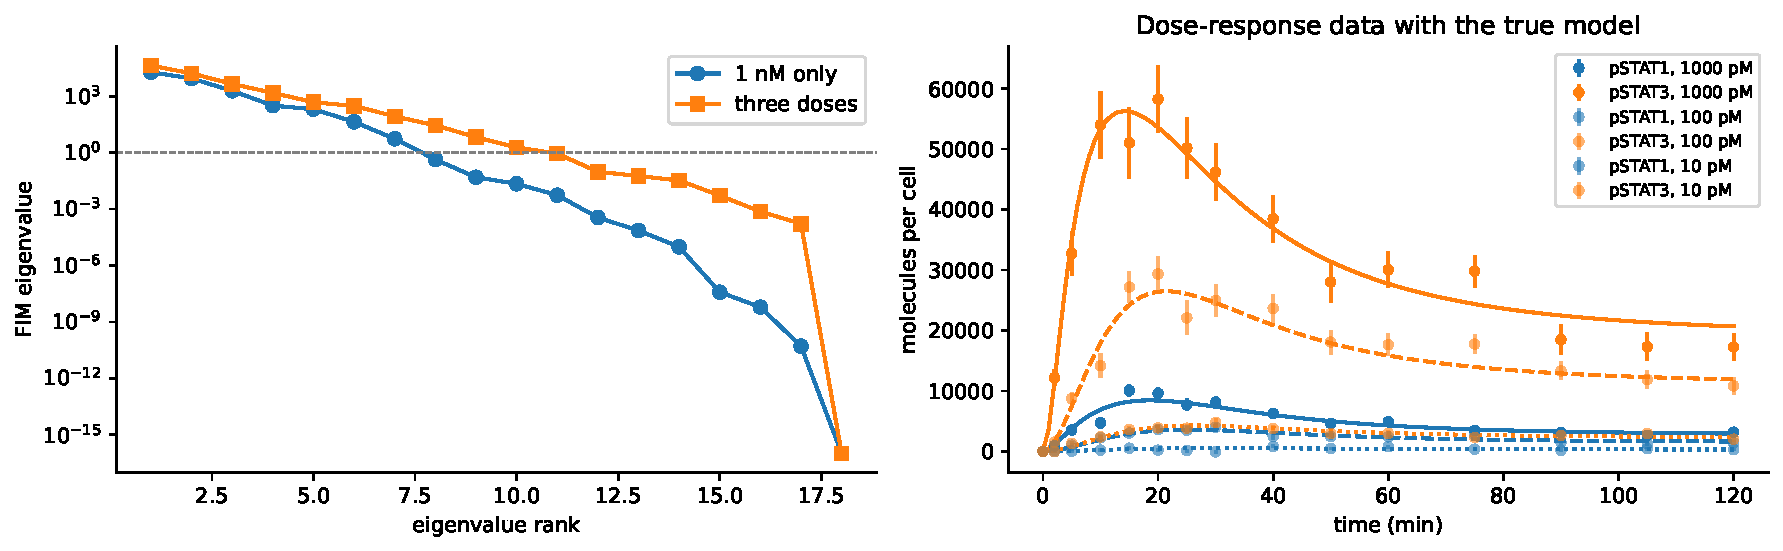
\includegraphics[width=0.95\linewidth]{design_fim.pdf}
  \raggedright
  \small
  \begin{itemize}[<2->]
    \item Add 100 pM and 10 pM doses: eigenvalues above 1 go from 7 to 10, and the
          sloppy directions gain several decades. \code{ktx}/\code{ktl} stays at zero.
  \end{itemize}
\end{frame}

\begin{frame}{More informative data, better estimates}
  \nbsection{8}
  \centering
  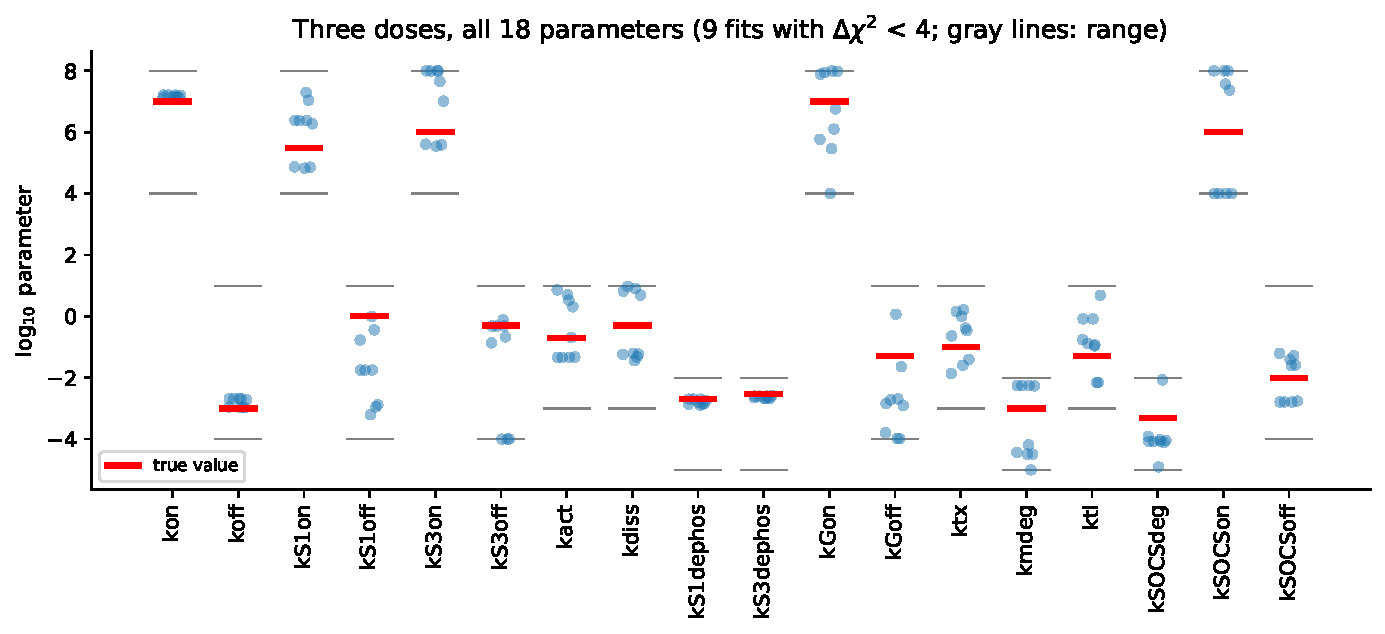
\includegraphics[width=0.76\linewidth]{recovery_all.pdf}
  \raggedright
  \small
  \begin{itemize}[<2->]
    \item \code{koff} moves from its bound to its true value; both dephosphorylation
          rates are pinned. The docking cycle is still undetermined: the next experiment
          should measure closer to it (receptor-bound STAT).
  \end{itemize}
\end{frame}

% ======================================================================
\begin{frame}{Try it yourself}
  \begin{columns}[T]
    \begin{column}{0.66\textwidth}
      Work through \code{notebooks/stat1\_stat3\_fitting.ipynb}, then:
      \begin{enumerate}
        \setlength\itemsep{1.5mm}
        \item Change the noise to 5\% and to 20\%. How do the FIM eigenvalues and
              the spread of good fits change?
        \item Replace \code{ktx} and \code{ktl} by their product. Is the product
              identifiable?
        \item Add total SOCS3 protein as a measured output. Which parameters become
              identifiable?
        \item Predict a SOCS3 knockout (\code{G0 = 0}) with each good fit. Do the fits
              agree? What does this say about predictions from a sloppy model?
      \end{enumerate}
    \end{column}
    \begin{column}{0.3\textwidth}
      \centering
      \qrcode[height=2.6cm]{\notebookurl}\\[1mm]
      {\scriptsize The notebook}
    \end{column}
  \end{columns}
\end{frame}

\begin{frame}{Summary}
  \begin{itemize}[<+->]
    \setlength\itemsep{2mm}
    \item Rate constants come in standard units; models of single cells often count
          \textbf{molecules}. Convert with $N_A V$, using the volume where the reaction
          happens.
    \item \textbf{Sensitivity analysis} finds the parameters that move the outputs:
          locally with derivatives, globally by sampling the plausible ranges.
    \item \textbf{Identifiability} concerns combinations of parameters. The FIM predicts
          which ones the data constrain, before fitting or even measuring.
    \item \textbf{Multistart fitting} finds the best fit, but many parameter sets fit
          equally well. Check \textbf{profiles} before trusting an estimate.
    \item Use the model to \textbf{design the next experiment}.
  \end{itemize}
\end{frame}

\begin{frame}{Additional reading}
  \small
  \begin{itemize}
    \setlength\itemsep{1.5mm}
    \item R.~N.~Gutenkunst et al.\ (2007). \textbf{Universally sloppy parameter
          sensitivities in systems biology models.} \emph{PLoS Comput.\ Biol.}\
          \textbf{3}, e189.
    \item A.~Raue et al.\ (2009). \textbf{Structural and practical identifiability
          analysis of partially observed dynamical models by exploiting the profile
          likelihood.} \emph{Bioinformatics} \textbf{25}, 1923--1929.
    \item S.~Marino et al.\ (2008). \textbf{A methodology for performing global
          uncertainty and sensitivity analysis in systems biology.} \emph{J.\ Theor.\
          Biol.}\ \textbf{254}, 178--196.
    \item E.~D.~Mitra and W.~S.~Hlavacek (2019). \textbf{Parameter estimation and
          uncertainty quantification for systems biology models.} \emph{Curr.\ Opin.\
          Syst.\ Biol.}\ \textbf{18}, 9--18.
    \item Y.~Sch\"alte et al.\ (2023). \textbf{pyPESTO: a modular and scalable tool for
          parameter estimation for dynamic models.} \emph{Bioinformatics} \textbf{39},
          btad711.
  \end{itemize}
\end{frame}

\end{document}
